%% ==================
\chapter{To go further: How to improve the model}
\label{ch:discussion}
%% ==================
%This chapter is dedicated to a discussion of the results obtained in the previous Chapter \ref{ch:results}.
%Discussions what do they mean?:


%%%FOLLOWING SECTION IS DONE IN RESULT CHAPTER AS WE PRESENT THE MCR, DM AND MSP RESULTS
%\section{Comparison of all 3 excess templates}
%	-Comparison of all 3 templates -> best is MCR from the chi2 maps
%		-Comparison MCR vs DM
%		-Comparison MCR vs MSP
%		-Weniger plots
%		-Specklings
%	

%\section{Interpretation of spatial shapes}
%	-Interpretation of spatial shapes
%		-Expected features
%			-PCR			
%			-IC spherical
%			-BR a little everywhere, less in bubbles			
%			-SCR in disk + bubbles
%		-Sandwich in IC and PCR
%			-MCR replaces PCR -> There is more MCs in disk. Blocks PCR
%			-IC in disk mostly due to Dust and starlight is blocked by it. Dust is only a small portion compared to starlight -> decrease
%		
%		-Shape of the excess component		
%			-Shape of MCR, DM, MSP -> traces the CO map
%			-Only make sense with MCR
%			-DM and MSP have no reason to do that


\section{Discussion on the spatial distributions of the other components.}

The spatial distribution of a component can teach a lot about the fit. Every component is closely linked to a known physical process taking place in the Milky way. So even if the components contributions to a single cone can not be predicted, large scale structures  should emerge and coincide with the predictions. Using this, it is possible to verify the proper functioning of the fit by comparing the fitted spatial distribution of the different templates and the predicted one.
For example, the distribution of the ISRF is expected to be spherical around the GC in the UV range, where most of the starlight is emitted. It can also follow the dust distribution in the disk in the infra-red range. This can be used to check if the IC component is coherent in the fit and follows, to some extent, the ISRF distribution. Hopefully, the results show a spherical IC component centred on the GC.
The different distributions of each component will be discussed in the following section.

\subsection{PCR flux distribution}
The PCR component is produced by diffuse CR protons which collide with other hadrons and form a neutral pion, which in turn decays into two photons. So the PCR flux is directly proportional to diffuse CR, gas and dust density in the galaxy along the line of sight. It is expected to be present in every direction, with a stronger flux coming from the disc, and less from high latitudes.
The bubbles have a harder CR proton spectrum, but composed of source protons. This could imply that more high energy pion are created in those regions, and so the PCR flux should be more important. But this is not true since the presence of the SCR component. The latter was created specifically for such regions with a hard CR spectrum and should take care of that instead of PCR. This way, PCR should not mark too much the bubbles shape.

The results are very similar for the three fits, with MCR, DM or MSP. The galactic disk is clearly visible at all longitudes, up to twenty degrees in latitude. Some structures from the gamma ray sky are also here, with the bulge around the GC and diffuse shapes at the anti-center.
Looking carefully at the disk below two degrees in latitude near the GC, the flux decreases a little, when it is supposed to be the highest. Indeed, the GC is were the density of matter along the line of sight is the most important, and so PCR should follow it. This structure could be interpreted as the result of a higher concentration of molecular clouds in this area, cutting off low energy CR, as modelled by MCR. This effect could affect the proportion of PCR gamma-rays in favour of MCR and reverse the relative contributions. Thus MCR should replace PCR, but the sum of both component should still show an increase in flux toward the GC. Indeed, the sum skymaps is coherent (see appendix \ref{app:PCR+MCR_integral_distribution}). Like for the bubbles, the propagated proton CR spectrum changes too much to be described by a single power law. If this interpretation is correct and it is not just a fitting mistake, it is an other argument that can easily be explained by the MCR hypothesis, but not by DM or MSP.


\begin{figure}[h]
  \centering
  \begin{minipage}[h]{0.45\textwidth}
  	\centering
	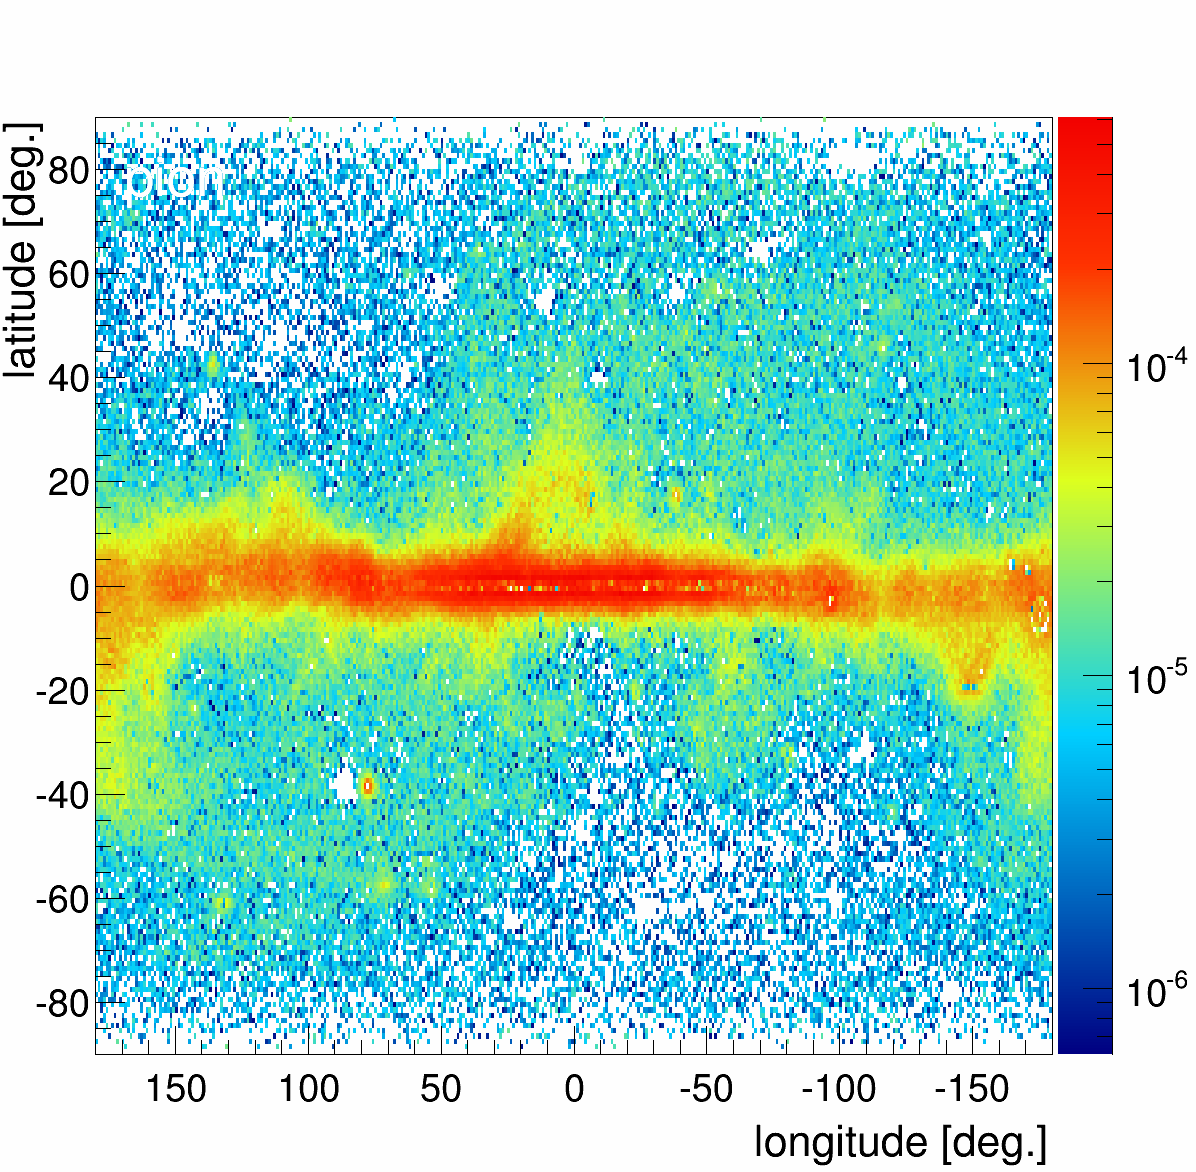
\includegraphics[width=1.\linewidth]{pic/discussion/MCRonly_fine_PCR_integral_distribution.png}
  	\subcaption{MCR}
  	\label{}
  \end{minipage}
  \hfill
  \begin{minipage}[h]{0.45\textwidth}
	  \centering
	  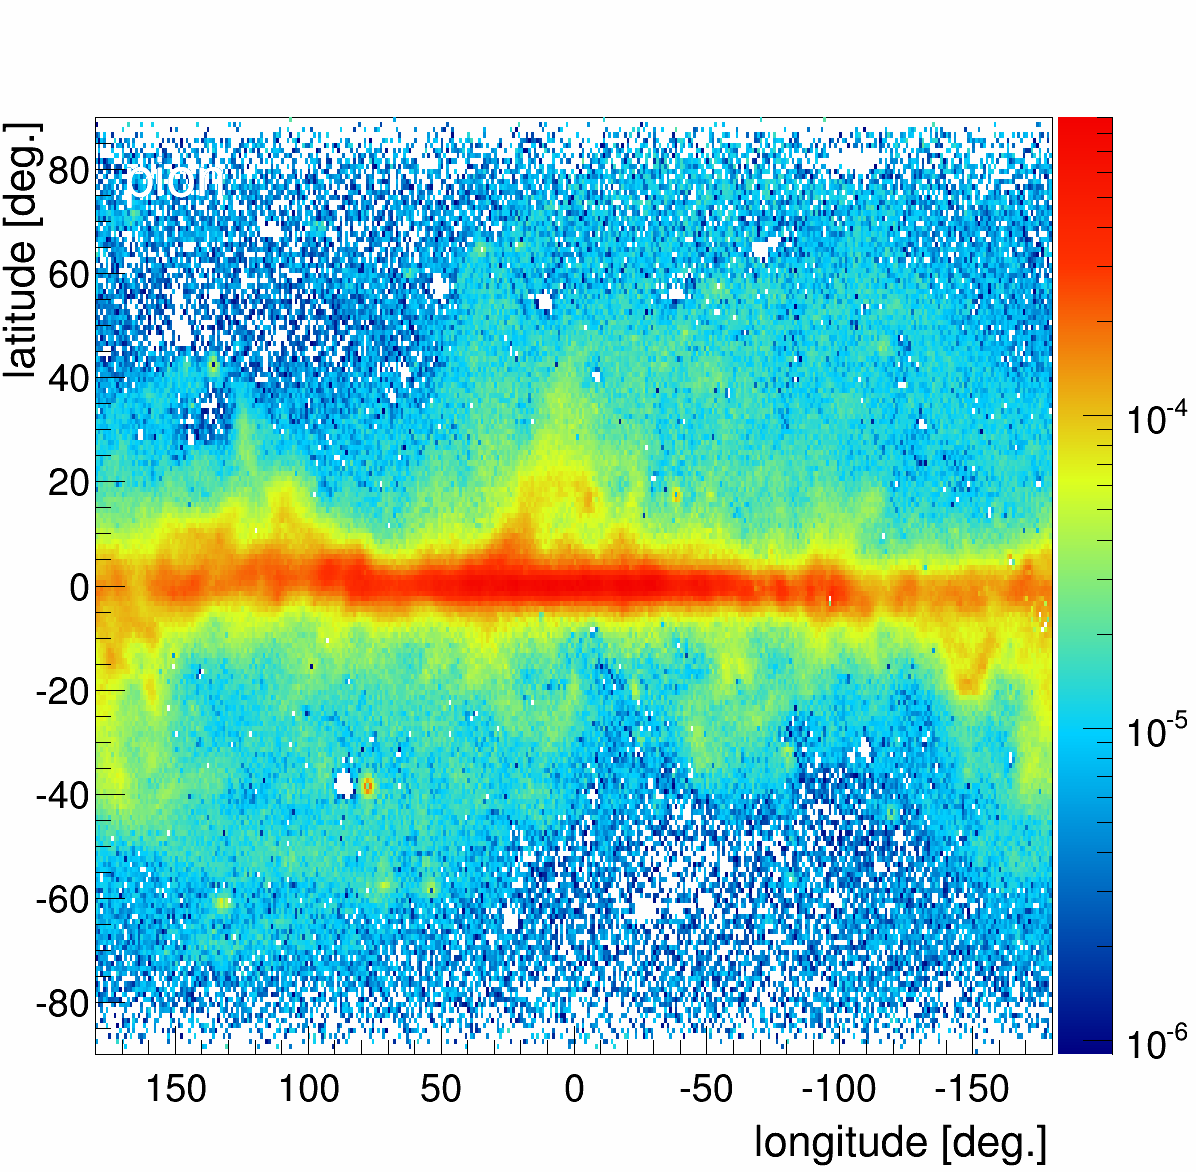
\includegraphics[width=1.\linewidth]{pic/discussion/DMonly_fine_PCR_integral_distribution.png}
	  \subcaption{DM}
	  \label{}
  \end{minipage}
  \hfill
  \begin{minipage}[h]{0.45\textwidth}
	  \centering
	  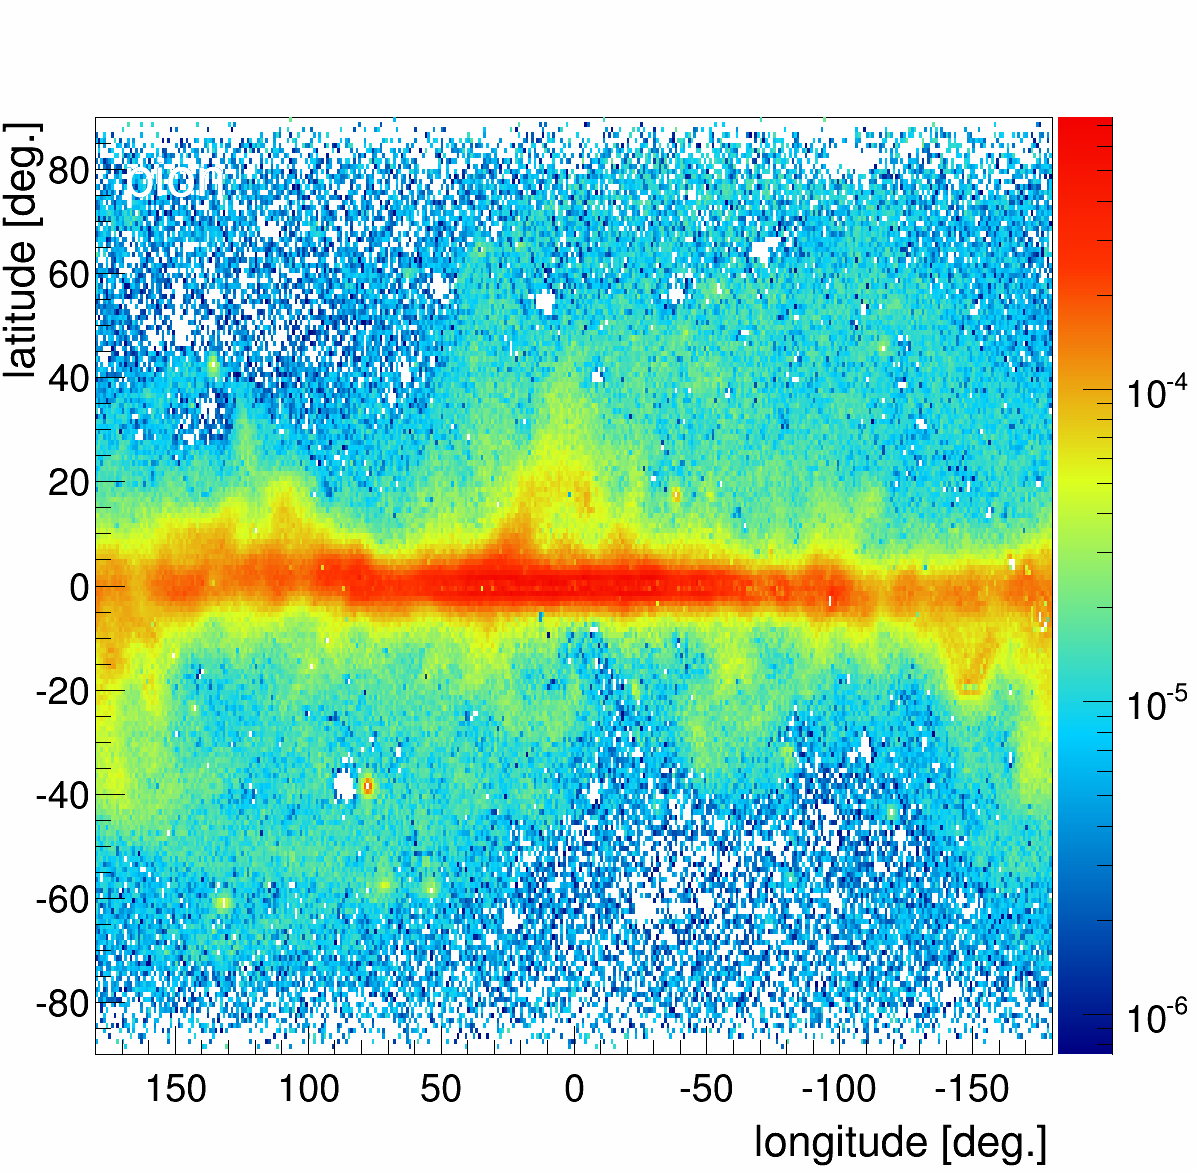
\includegraphics[width=1.\linewidth]{pic/discussion/MSPonly_fine_PCR_integral_distribution.png}
	  \subcaption{MSP}
	  \label{}
  \end{minipage}
  \caption[PCR spatial distributions.]{PCR spatial distribution with a MCR (a), a DM (b) and a MSP (c) fit. The galaxy disk and matter distribution is clearly visible. With MCR and to a lesser extend MSP, a drop in flux can be observed in the disk, below two degrees in latitude. This could be the excess component tracing MCs that take other PCR, tracing the propagated CRs.}
  \label{fig:PCR_flux_distrib_excess_comp}	 
\end{figure}


\newpage
\subsection{IC flux distribution}
The inverse compton scattering component is directly proportional to the ISRF and the electrons CR. Electrons are present everywhere in the galaxy, and the ISRF is dominant in the GC for the UV range, but follows the dust in the IR range and is isotropic in the radio. This distribution should be visible in the IC component of the fit.
Indeed, a spherical distribution can clearly be identified for the three different fits with DM, MCR and MSP. Nonetheless, there is a noticeable difference in the disk between the IC distribution for the MCR and DM fits and the MSP fit. In the MCR and DM fit, the disk presents a high IC flux when and MSP does not. On the contrary, the MSP fit presents a clear dip in the galactic disk. This gap is unexpected, since the ISRF is supposed to be the strongest in the disk, and the diffuse electrons are also produced mainly here. This effect could come from the shape of the MSP spectrum at low energies. Indeed, being softer than MCR and DM, and having a higher contribution in the disk where the excess is present, the fit overshoot the low energies under 1 GeV. This does not leave any space for an IC component that is also very soft. This is sown in figure \ref{fig:Excess_comp_comparison} where the only fit that does not need IC in the CMZ is the MSP fit.

\begin{figure}[h]
  \centering
  \begin{minipage}[h]{0.45\textwidth}
  	\centering
	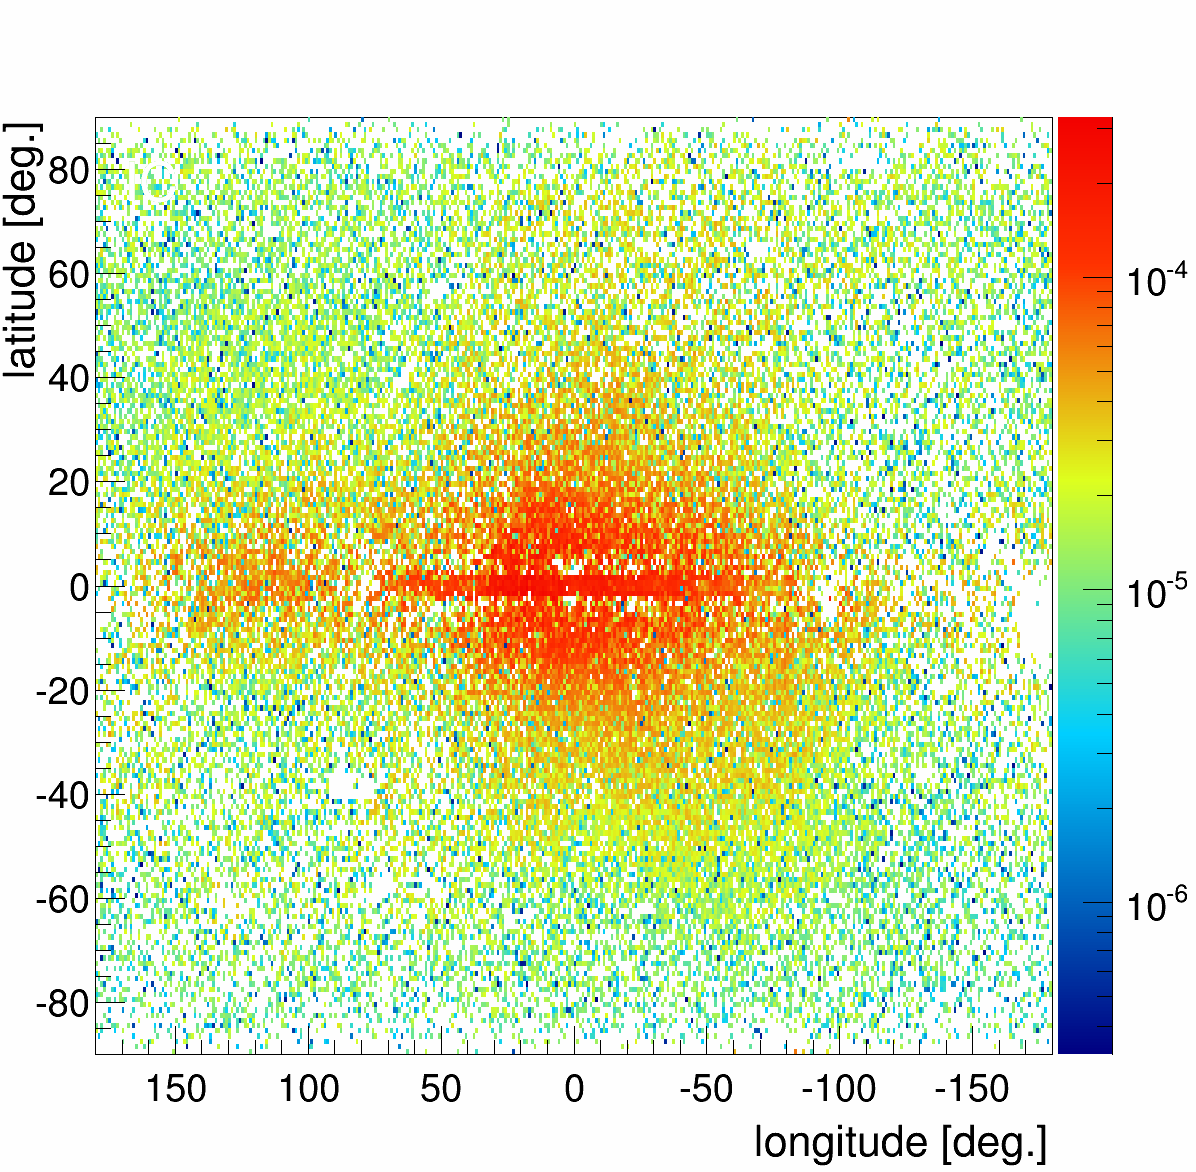
\includegraphics[width=1.\linewidth]{pic/discussion/MCRonly_fine_IC_integral_distribution.png}
  	\subcaption{MCR}
  	\label{}
  \end{minipage}
  \hfill
  \begin{minipage}[h]{0.45\textwidth}
	  \centering
	  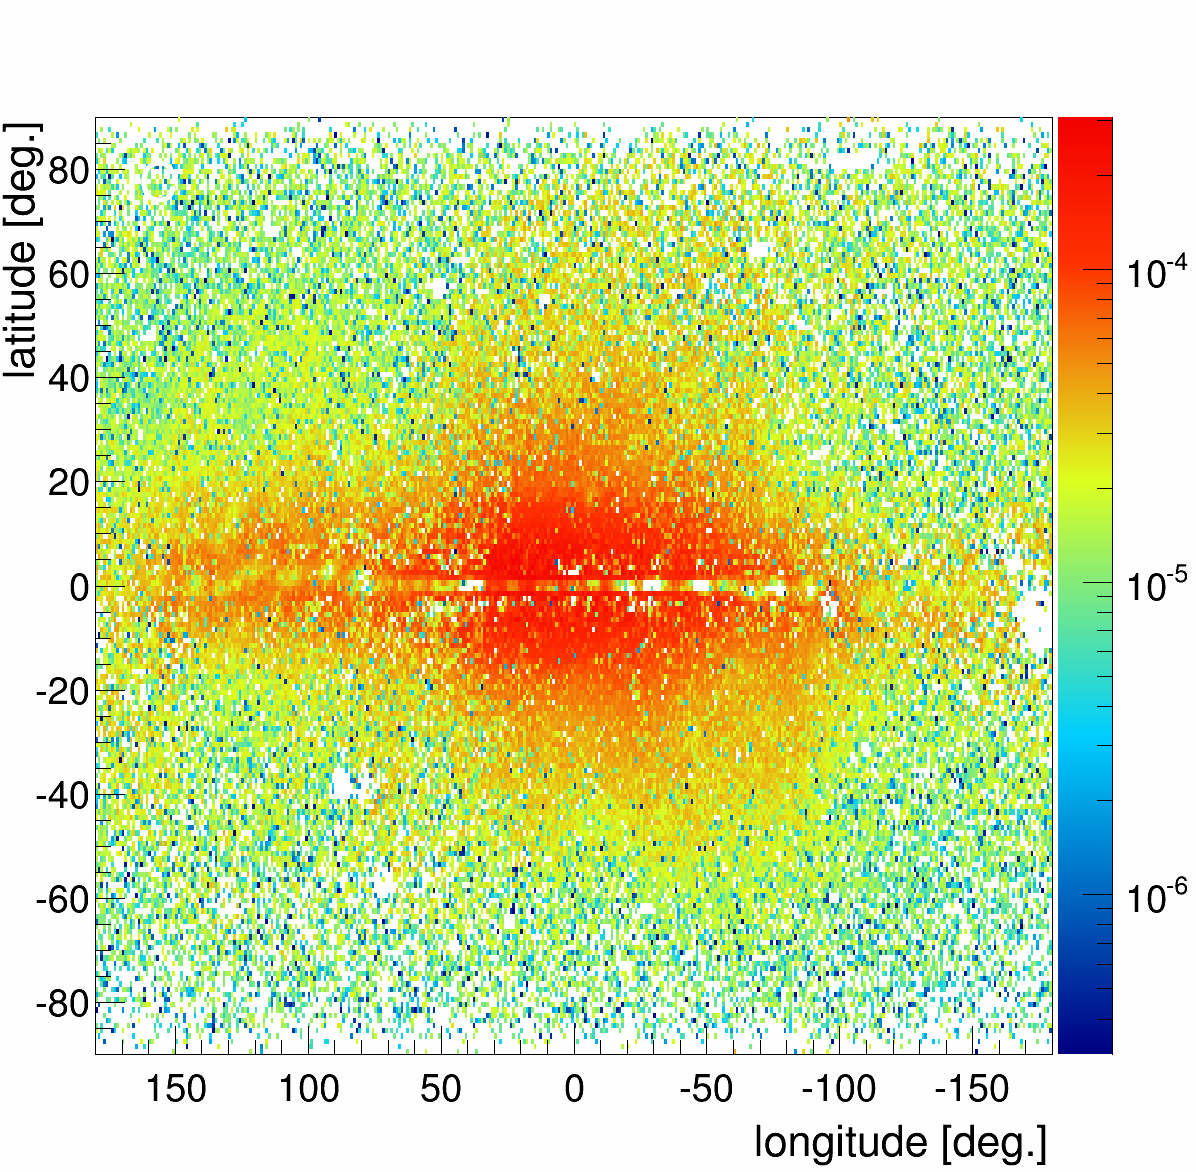
\includegraphics[width=1.\linewidth]{pic/discussion/DMonly_fine_IC_integral_distribution.png}
	  \subcaption{DM}
	  \label{}
  \end{minipage}
  \hfill
  \begin{minipage}[h]{0.45\textwidth}
	  \centering
	  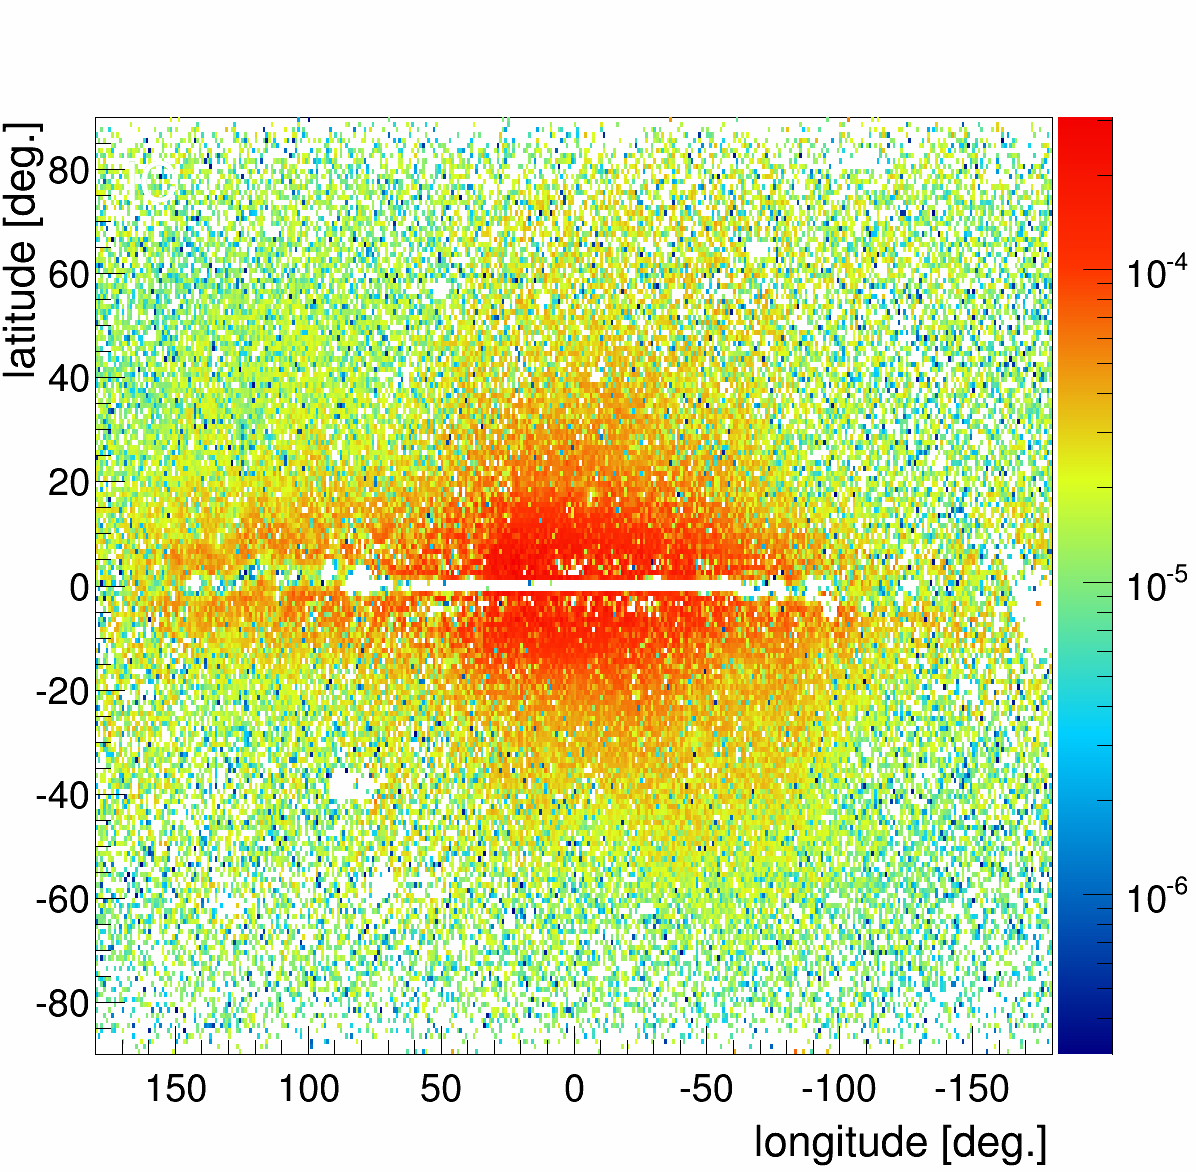
\includegraphics[width=1.\linewidth]{pic/discussion/MSPonly_fine_IC_integral_distribution.png}
	  \subcaption{MSP}
	  \label{}
  \end{minipage}
  \caption[IC spatial distributions.]{IC spatial distribution with a MCR (a), a DM (b) and a MSP (c) fit.}
  \label{fig:IC_flux_distrib_excess_comp}	 
\end{figure}

\newpage
\subsection{BR flux distribution}
The BR component is linked to the CR electron density along the line of sight and the gas distribution in the galaxy. It should then be present everywhere. It is what can be observed in Fig. \ref{fig:BR_flux_distrib_excess_comp}, but some features are remarkable. Mainly the decrease of the flux in the disk and the bubbles.
Depending on the fit, the average flux is also changing. The BR component is a lot more present with the MCR fit than with DM, which in turn presents more BR than the MSP fit. The fact that the MSP fit does not use a lot of BR is consistent with the fact that the MSP spectrum is very soft at low energies. Since BR is also dominant at these energies, both cannot have a high flux at the same time. The fit must do concession in order to use them both.

\begin{figure}[h]
  \centering
  \begin{minipage}[h]{0.45\textwidth}
  	\centering
	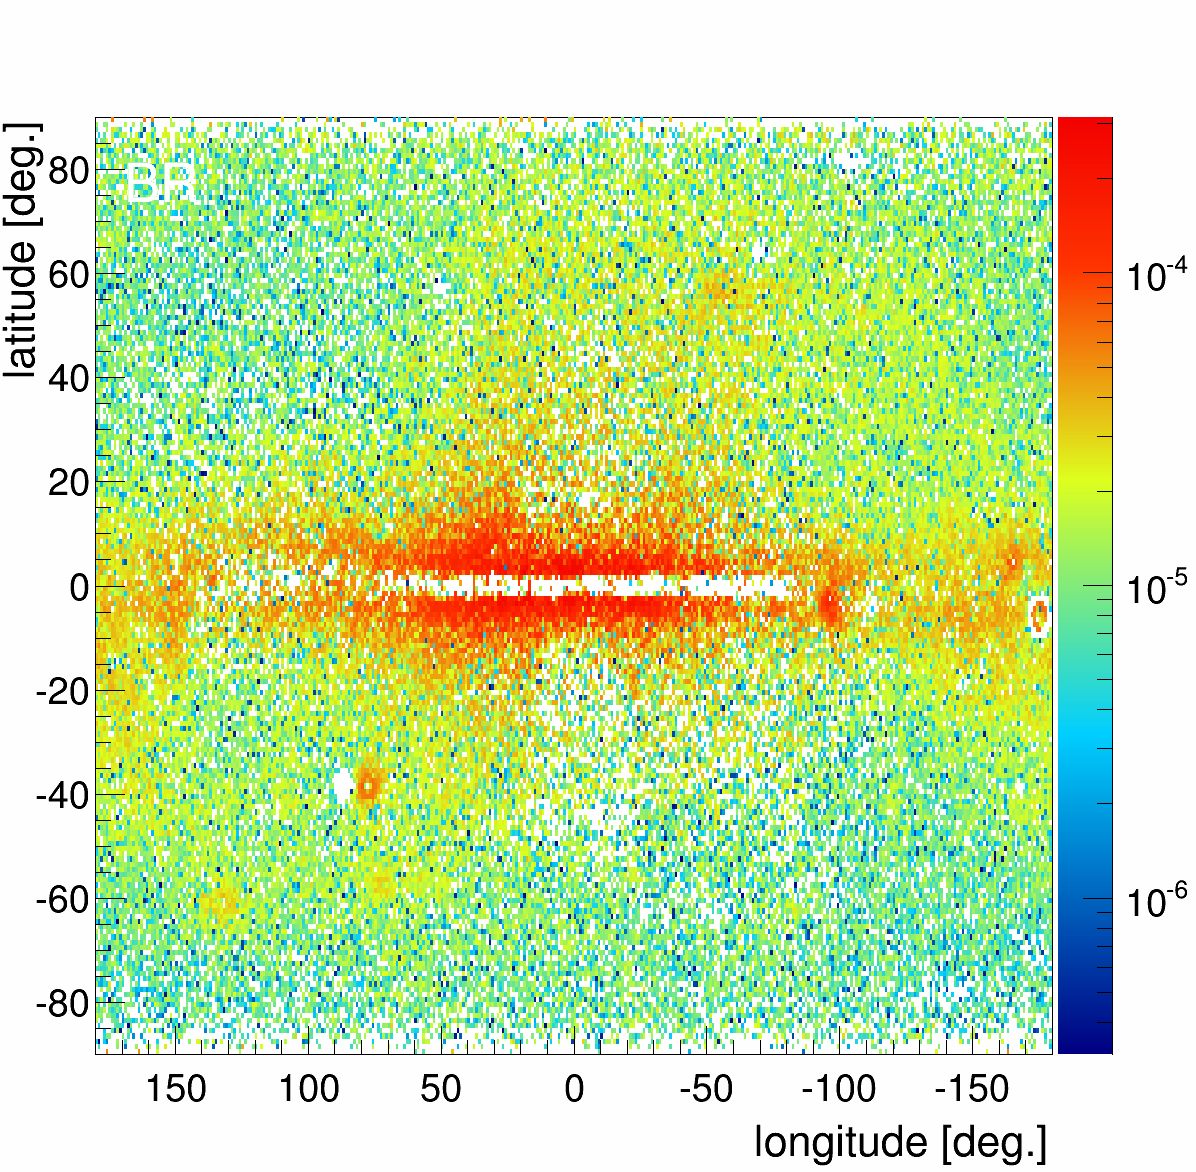
\includegraphics[width=1.\linewidth]{pic/discussion/MCRonly_fine_BR_integral_distribution.png}
  	\subcaption{MCR}
  	\label{fig:MCRonly_BR_dist}
  \end{minipage}
  \hfill
  \begin{minipage}[h]{0.45\textwidth}
	  \centering
	  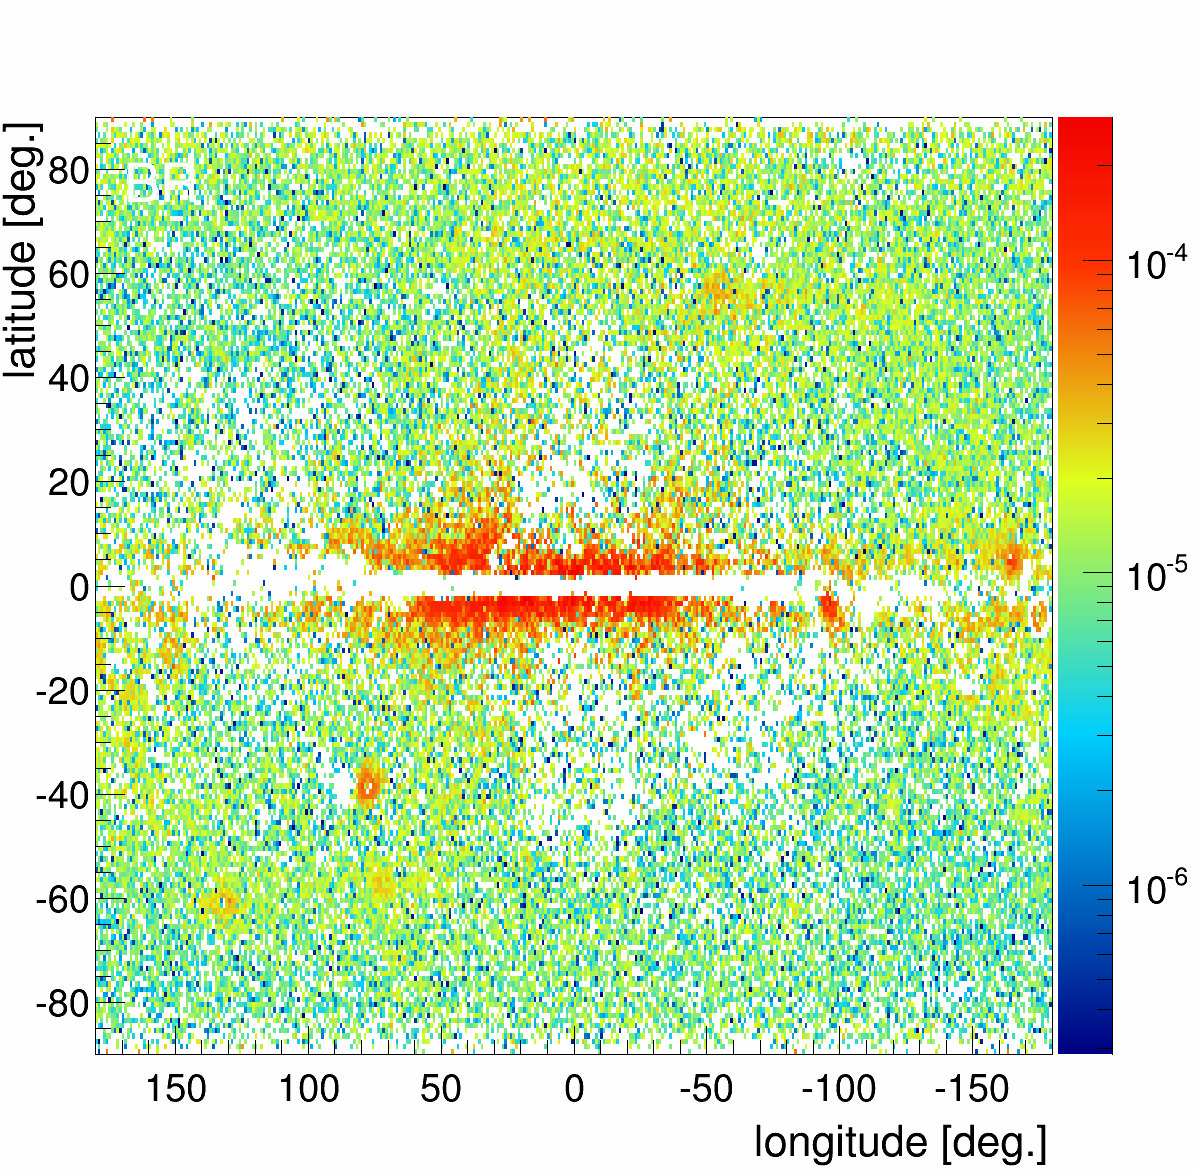
\includegraphics[width=1.\linewidth]{pic/discussion/DMonly_fine_BR_integral_distribution.png}
	  \subcaption{DM}
	  \label{}
  \end{minipage}
  \hfill
  \begin{minipage}[h]{0.45\textwidth}
	  \centering
	  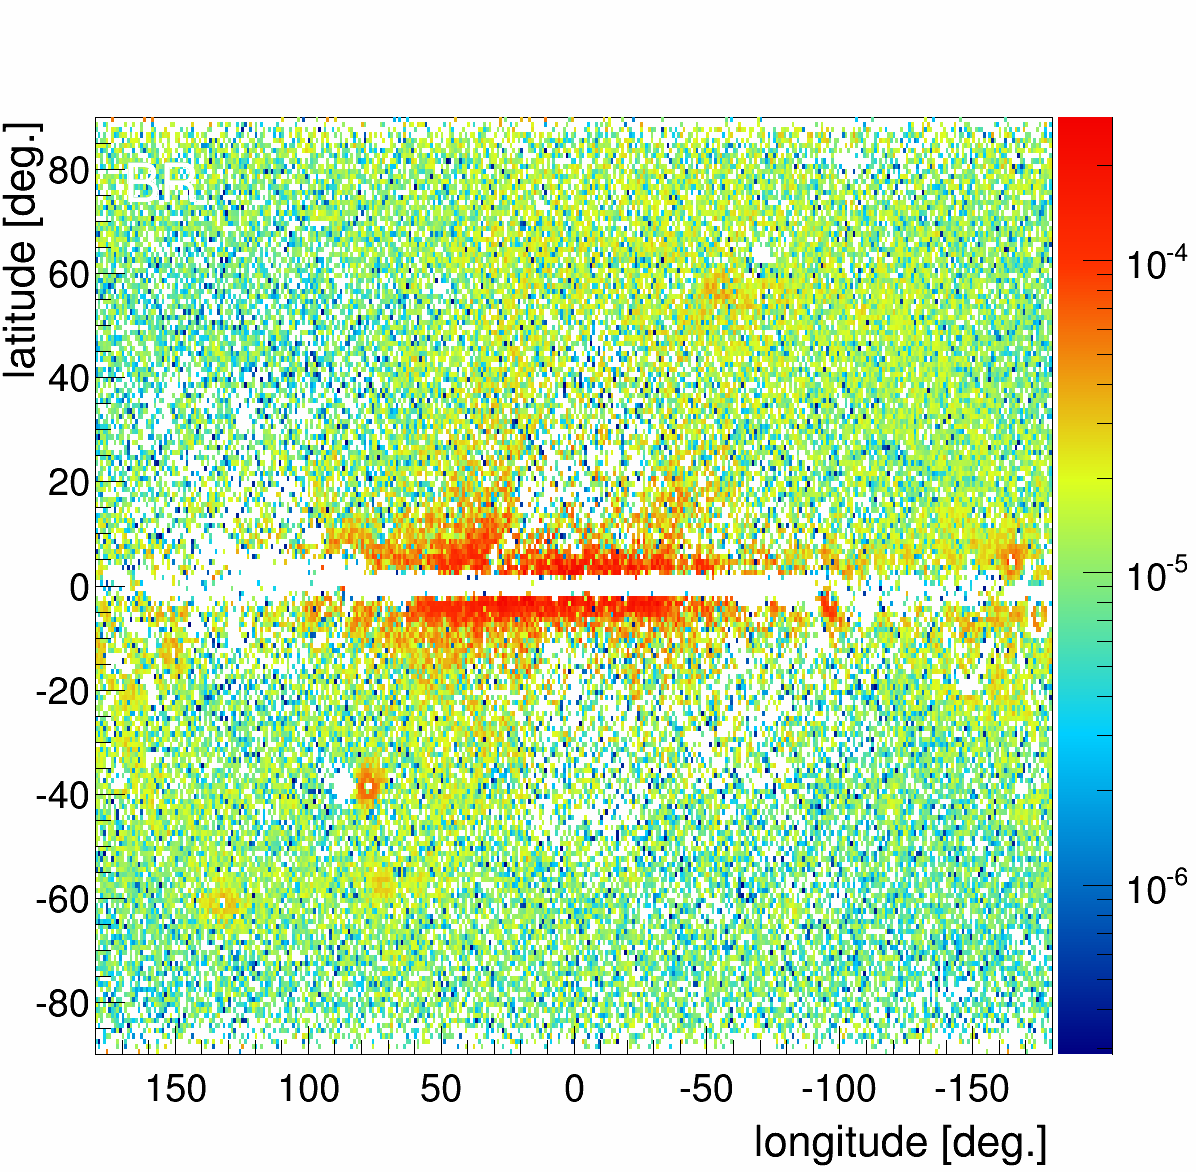
\includegraphics[width=1.\linewidth]{pic/discussion/MSPonly_fine_BR_integral_distribution.png}
	  \subcaption{MSP}
	  \label{}
  \end{minipage}
  \caption[BR spatial distributions.]{BR spatial distribution with a MCR (a), a DM (b) and a MSP (c) fit.}
  \label{fig:BR_flux_distrib_excess_comp}	 
\end{figure}
\newpage
\subsection{SCR flux distribution}
The SCR distribution is expected to follow the disc, where point sources can still remain, and the bubbles, where the proton CR spectra is harder. And indeed, the spatial distribution obtained in the three  different fits are similar and correspond perfectly to the expectations.


\begin{figure}[h]
  \centering
  \begin{minipage}[h]{0.45\textwidth}
  	\centering
	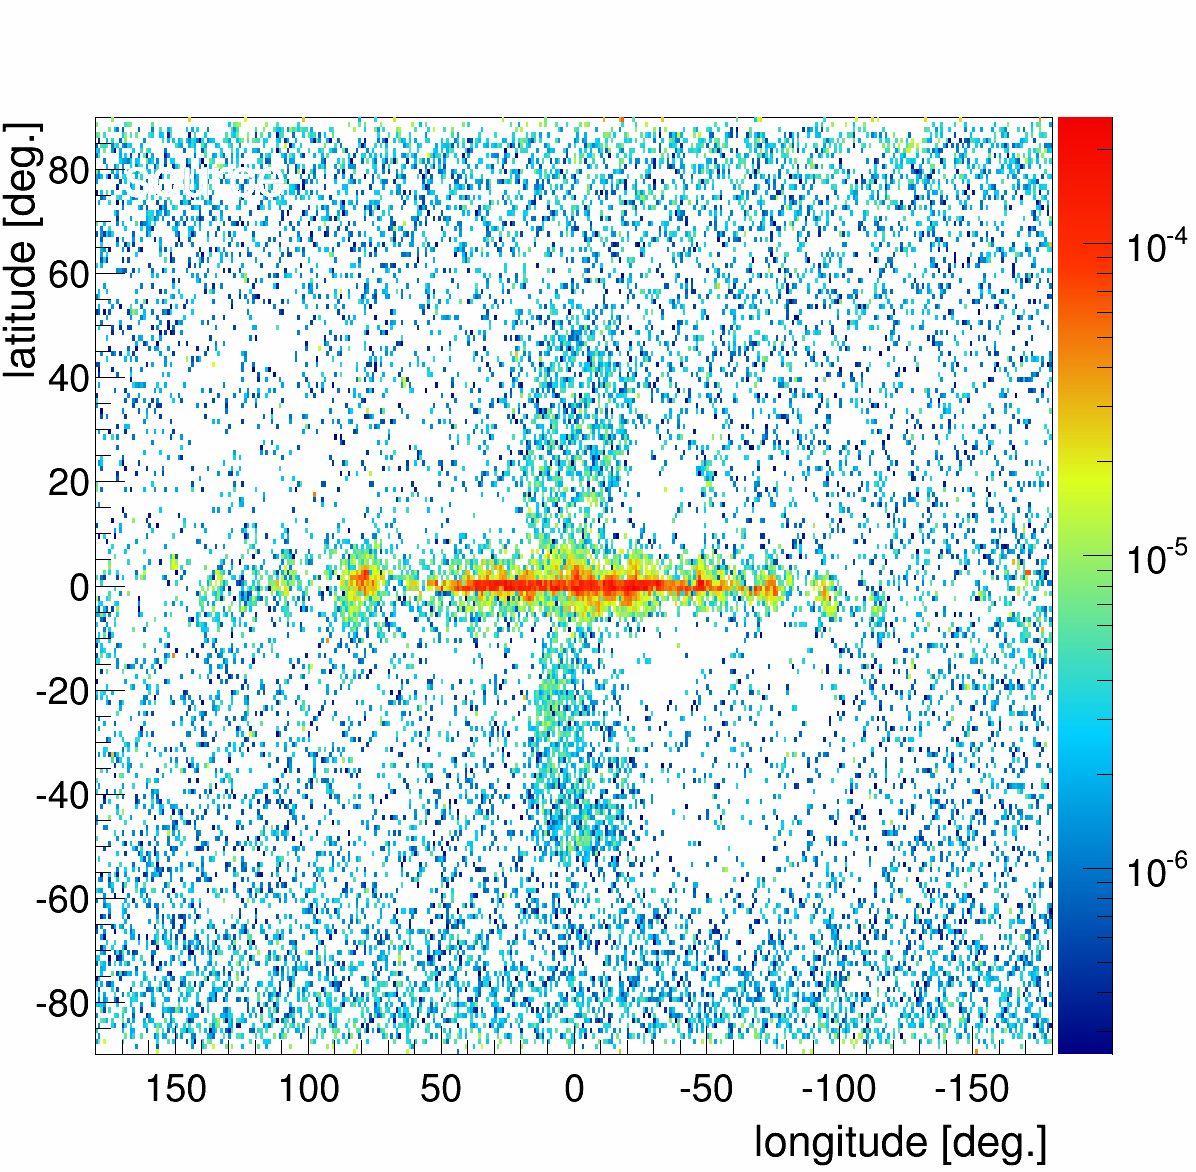
\includegraphics[width=1.\linewidth]{pic/discussion/MCRonly_fine_SCR_integral_distribution.png}
  	\subcaption{MCR}
  	\label{}
  \end{minipage}
  \hfill
  \begin{minipage}[h]{0.45\textwidth}
	  \centering
	  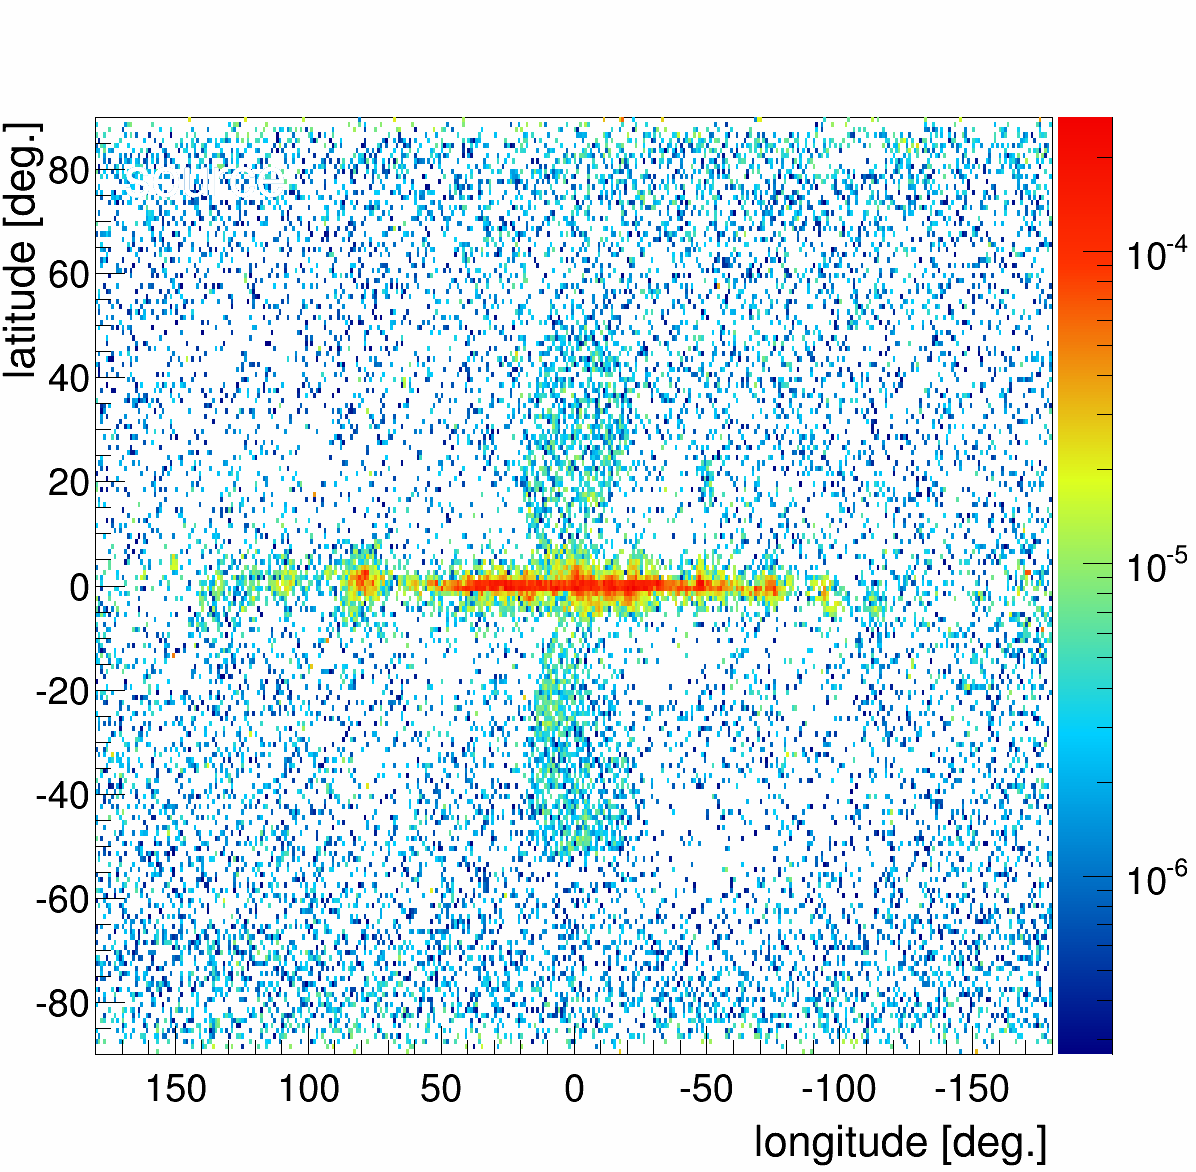
\includegraphics[width=1.\linewidth]{pic/discussion/DMonly_fine_SCR_integral_distribution.png}
	  \subcaption{DM}
	  \label{}
  \end{minipage}
  \hfill
  \begin{minipage}[h]{0.45\textwidth}
	  \centering
	  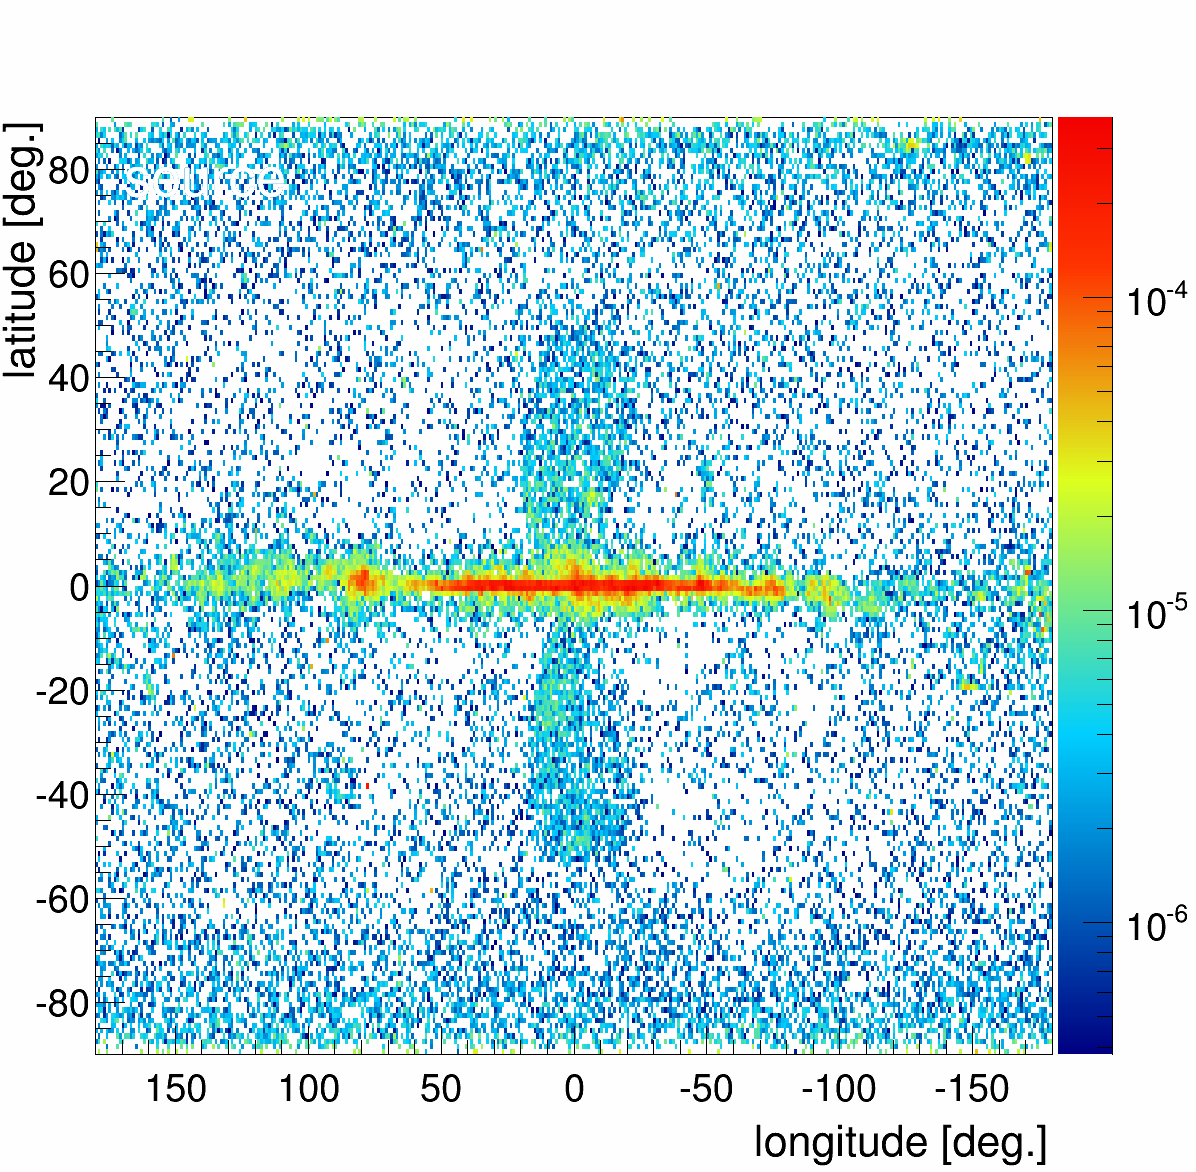
\includegraphics[width=1.\linewidth]{pic/discussion/MSPonly_fine_SCR_integral_distribution.png}
	  \subcaption{MSP}
	  \label{}
  \end{minipage}
  \caption[SCR spatial distributions.]{SCR spatial distribution with a MCR (a), a DM (b) and a MSP (c) fit.}
  \label{fig:SCR_flux_distrib_excess_comp}	 
\end{figure}



\newpage
\section{Adding an break in electron CR spectrum}

The theory behind the MCR component involves a magnetic cut-off for low rigidity CR protons that changes the gamma-ray spectrum at low energies. Such a cut-off only depends on the rigidity of the CR and the intensity of the electromagnetic field. So there is no reason for it to be only applied to protons, and not to electrons. This is the reasoning that led to the introduction of a new template, called MBR in the fit, equivalent to the BR template, but calculated from a different electron CR spectrum.
This new CR spectrum is composed of two different power laws for high and low energies, joining at the break position. It has the exact same spectral indexes than the CR spectrum used for IC and BR (0.81 below and 3.21 above), but the break is moved up, between 6 and 14 GeV, to stay consistent with the MCR break. The fit method is the same, and the MBR break is fixed to the MCR brake in a given region. This way, the magnetic cut-off is applied the same way to the electrons and protons CR in the same region. Once again, this component is expected to follow the MCs distribution, as expected with MCR.

A MIC component was tested as well, but it was not kept in the fit. This component would have been an IC component with a break between 6 and 14 GeV in the electron spectrum, following the same reasoning than for MBR.
The reason it was not kept is that it did not improve the fit at all. It is very close from the initial IC component, and do not bring anything new.

Figure \ref{fig:MBR_results} shows the results of such a fit and its effect on the BR component. As with the MCR fit \ref{fig:MCRonly_CMZ_1}, the CMZ is very well fitted by the model. There is still no BR contribution, but MBR template is present. The spatial distribution of BR is also very similar to the MCR fit (see Fig. \ref{fig:MCRonly_BR_dist}), with a lower flux in the disk and the bubbles. On the contrary, the MBR component is mainly present in the disk and the GC, as expected, where MCs are supposed to change the electron CR spectrum. The bubbles also appear to show a MBR contribution that is not predicted by the theory behind MBR. This can be interpreted as a hint that the model is not perfect, and that the different templates do not only play their theoretical role, but can also be used where they are not supposed to. In that case, a fine tuning of the CR spectra used to get the gamma-rays templates is required to get the theoretical distributions.


\newpage
\begin{figure}[H]
  \centering
  \begin{minipage}[h]{0.45\textwidth}
  	\centering
	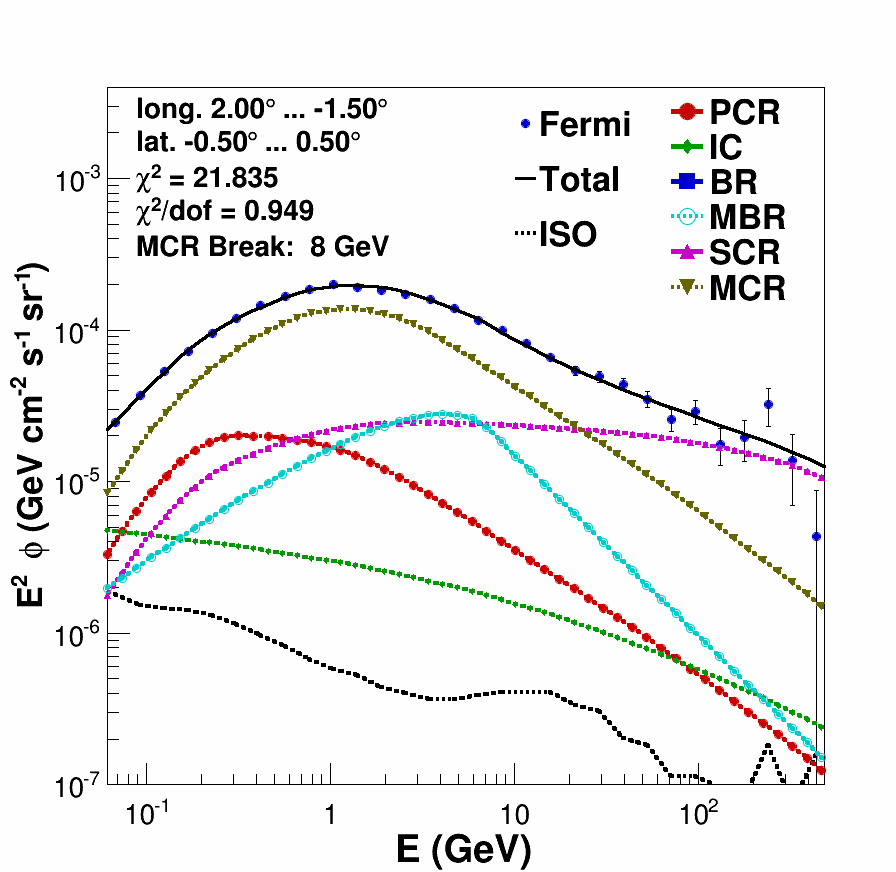
\includegraphics[width=1.\linewidth]{pic/discussion/MBR_CMZ.png}
  	\subcaption{}
  	\label{}
  \end{minipage}
  \hfill
  \begin{minipage}[h]{0.45\textwidth}
	  \centering
	  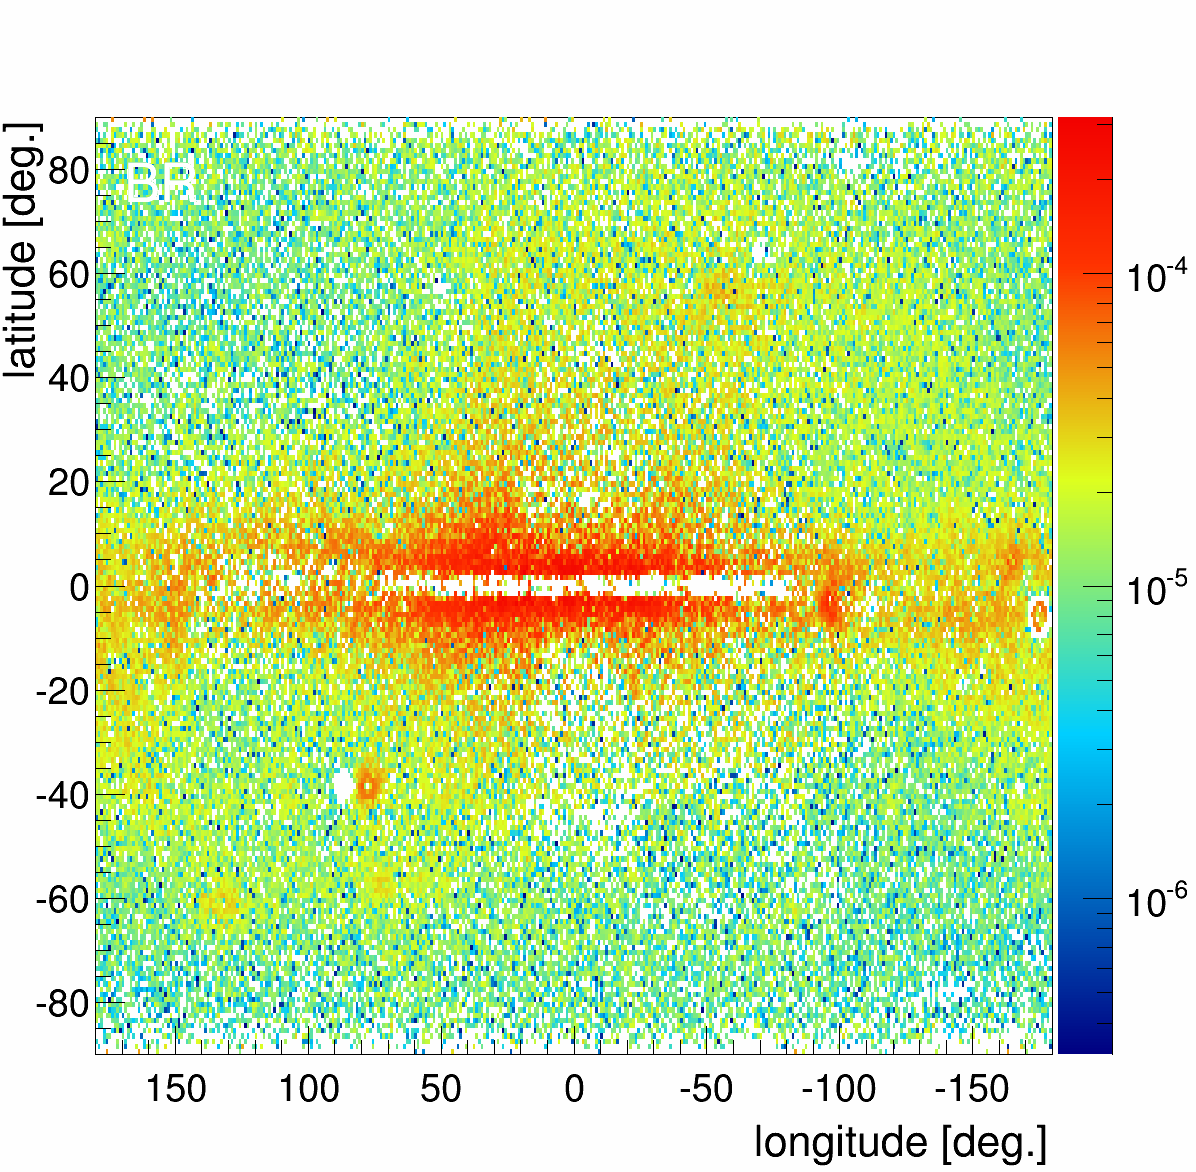
\includegraphics[width=1.\linewidth]{pic/discussion/MBR_BR_Integral.png}
	  \subcaption{}
	  \label{}
  \end{minipage}
  \hfill
  \begin{minipage}[h]{0.45\textwidth}
	  \centering
	  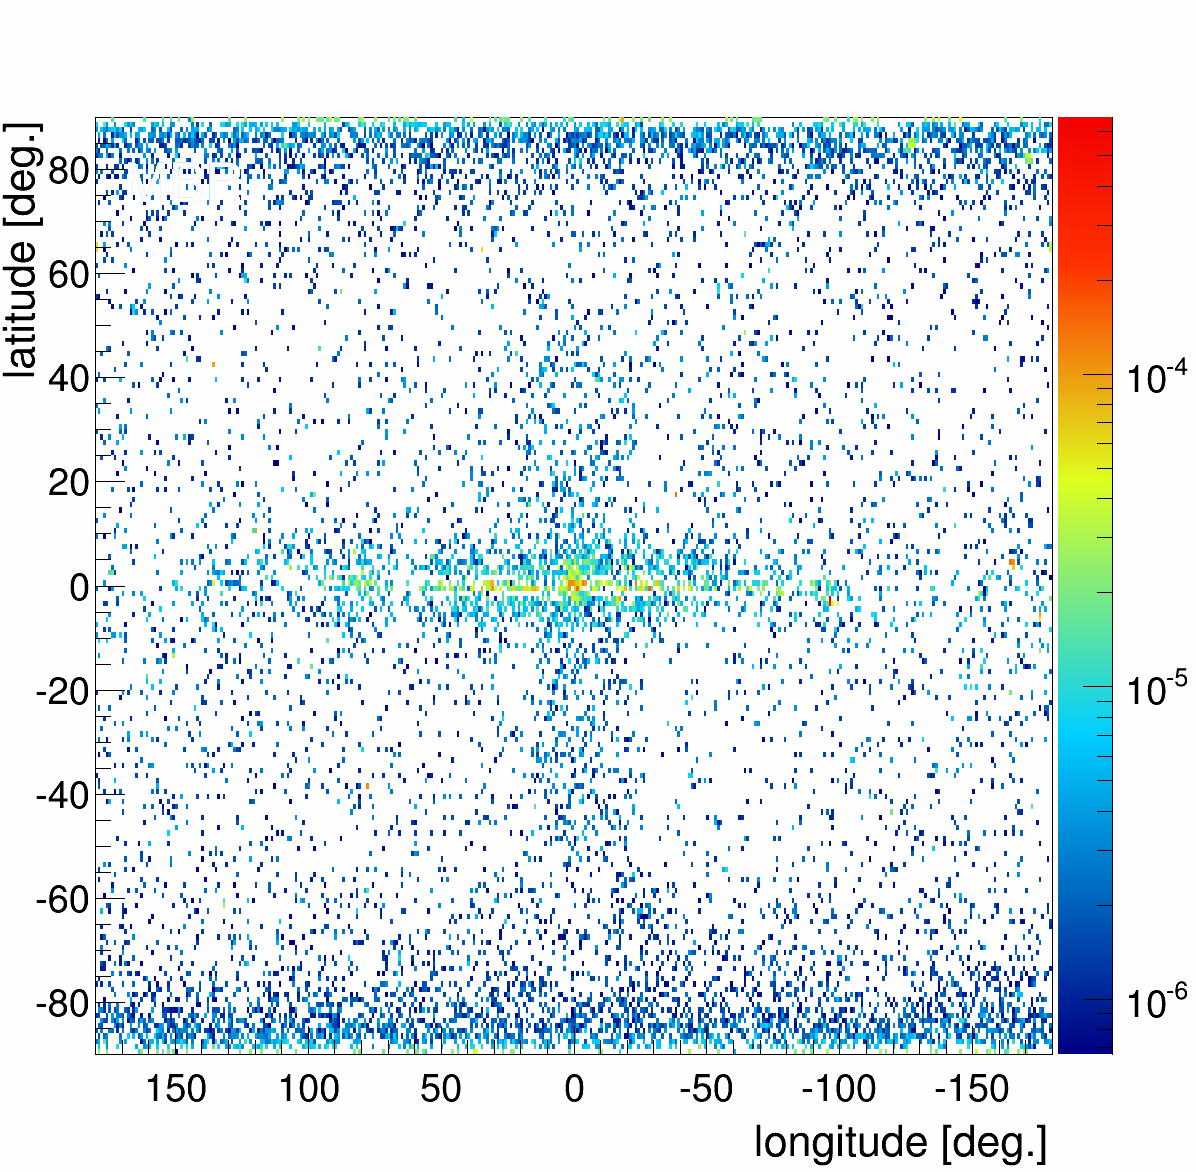
\includegraphics[width=1.\linewidth]{pic/discussion/MBR_MBR_Integral.png}
	  \subcaption{}
	  \label{}
  \end{minipage}
  \hfill
  \begin{minipage}[h]{0.45\textwidth}
	  \centering
	  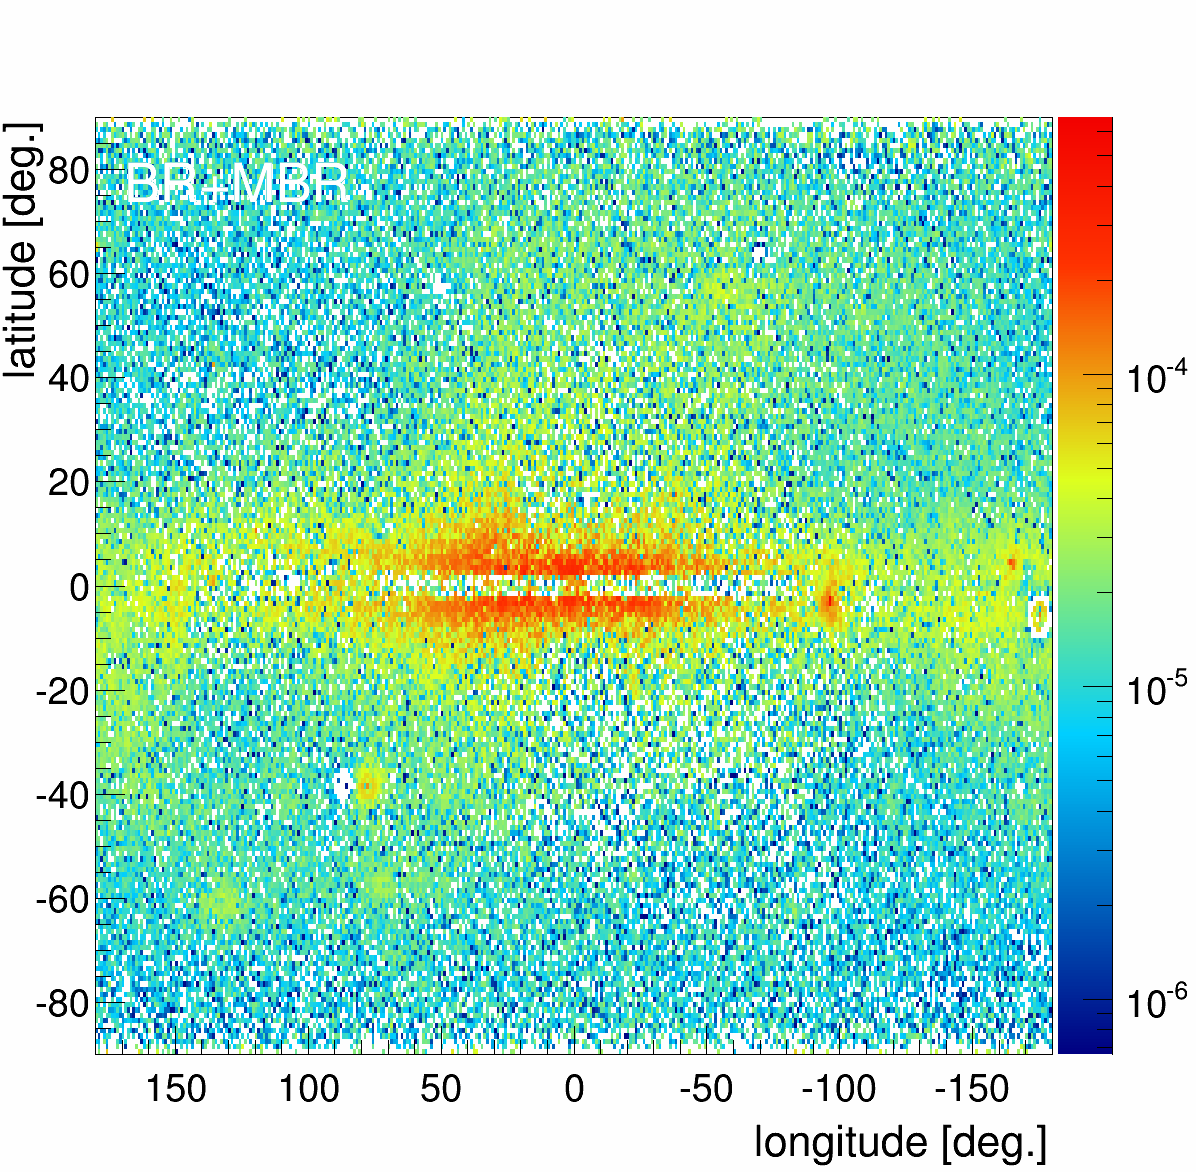
\includegraphics[width=1.\linewidth]{pic/discussion/MBR_BR+MBR_Integral.png}
	  \subcaption{}
	  \label{}
  \end{minipage}
  \caption[Results of the fit with MBR]{Results of the fit using a MBR component. (a) CMZ spectrum. The MBR component has a major contribution around 5 GeV. Compared to Fig. \ref{fig:MCRonly_CMZ}, the fit slightly improves with a smaller $\chi^2$ value. (b) BR flux distribution. It resembles closely the distribution before adding MCR, with a strong gap in the disk (see Fig. \ref{fig:MCRonly_BR_dist}). (c) MBR flux distribution. It is strong in the GC and the disk, but decreases rapidly around. The pole structures are artifacts due to a lack of statistics at high latitudes. (d) Sum of BR (b) and MBR (c) flux. The MBR contribution is not strong enough to fill the BR gap in the disk.}
  \label{fig:MBR_results}	 
\end{figure}




\newpage
\section{Mixing MCR and DM}

Now the results are clear. MCR is a good solution to the gamma-ray GeV excess in the GC, and could replace the first hypotheses of a DM halo or hidden MSPs. Yet, the DM theory is strongly supported by other measurements, for example the rotation curves of galaxies  \cite{Newby2018} \cite{Rubin1971}, and is one of the most important question of modern physics. And the fact that it is not the primary cause of the effect observed here does not mean it does not exist. On the contrary, under the hypothesis that MCR is really the cause of the excess, the fit could put strong limits on the DM models.

This section will present a few ways to study the current DM WIMP model using the fit method of this thesis.


\subsection{DM and MCR in the same fit}

A first idea is to give the fit a DM and a MCR template with free scaling factors and let it combine them to find the best $\chi^2$ value. Taking a 52.3 GeV WIMP mass and the MCR template with free breaks between 6 and 14 GeV, the fit has the choice between the two. 
The results are in favor of MCR (Fig \ref{fig:DM+MCR_distribution}), almost ignoring the DM component. This could be predicted from the previous comparisons of the $\chi^2$ distribution for a MCR or a DM fit that showed a clear preference toward MCR, at least in the disk. Furthermore, the $\chi^2$ map of a MCR fit is flat around one, even in the disk, whereas a DM fit does not work well for small latitudes. Here the contribution of DM is very small, and the results are almost an exact copy of the fit with MCR only as the excess component.

\begin{figure}[H]
	\centering
	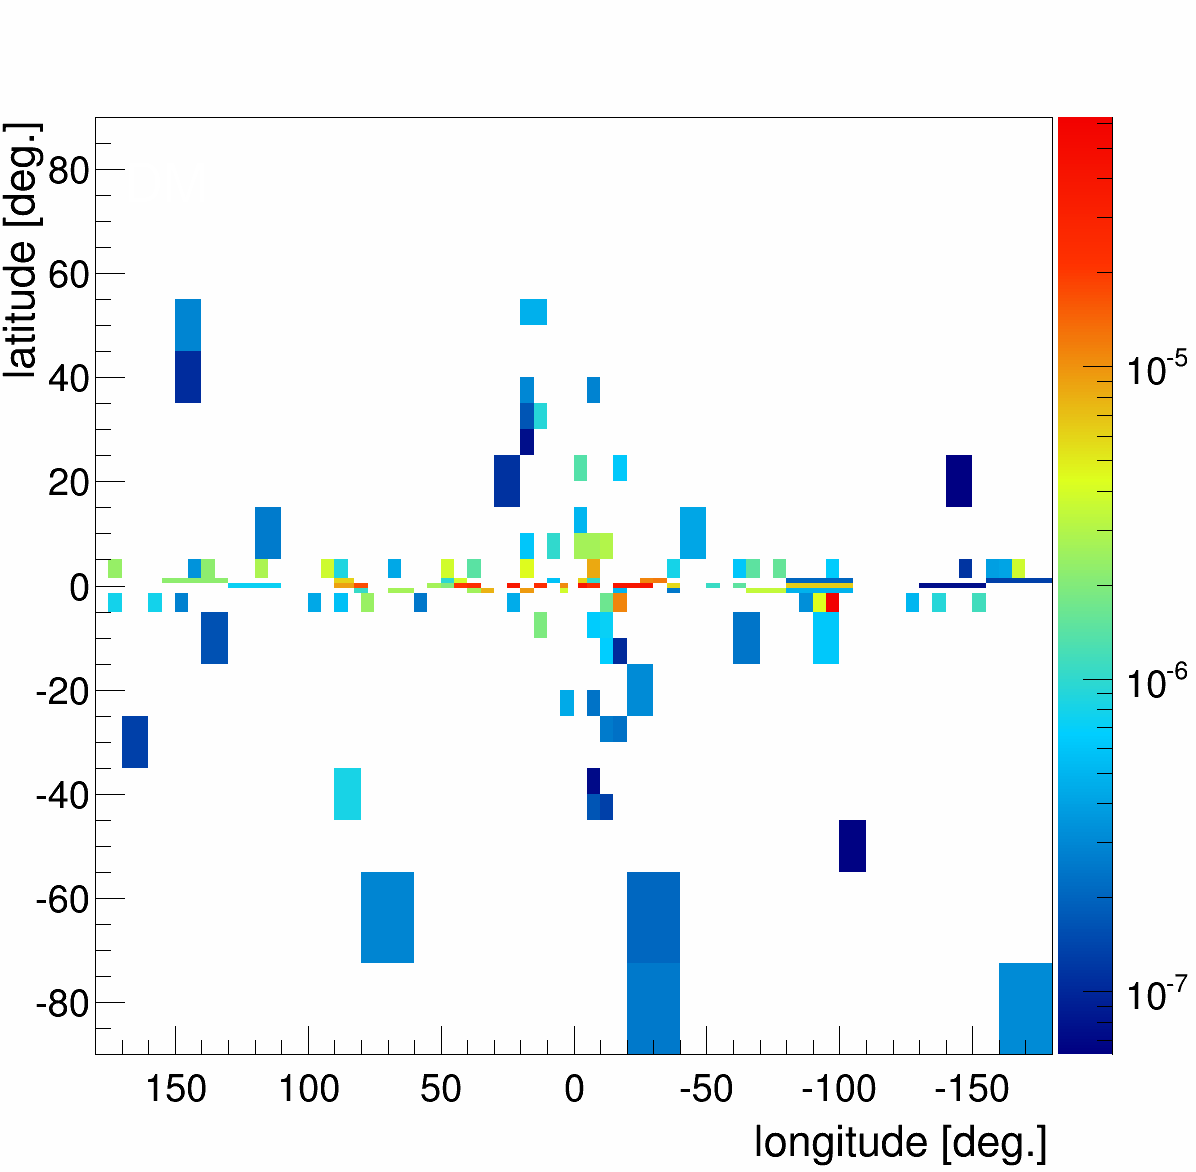
\includegraphics[width=.5\linewidth]{pic/discussion/DM+MCR_DM_distribution.png}
	\caption[DM distribution for a fit using DM and MCR]{DM flux distribution fitting all background components, SCR, MCR and DM. DM is almost not used anywhere, thus using DM or not does not change the results of the fit. The adapted binning of 797 cones is used here because the statistics are too low in a one by one degree binning to show the DM contribution.}
	\label{fig:DM+MCR_distribution}
\end{figure}

\newpage
\subsection{Adding DM afterwards}

The second idea that comes to mind is to take the MCR template for granted, and see if there is space to add a DM contribution after fitting with MCR. In other words, a first fit is performed with the classical templates (PCR, IC, BR), the source (SCR) and the MCR templates. Once the best $\chi^2$ is found, the fit tries to add a DM template to improve the model.
Following the Ockham's razor principle, the least amount of contributions are accepted as true, and any additional component must be treated carefully. This way, the necessity of a DM template is checked, and its contribution can not be mistaken for a classical one.

The results are clear, the fit adds only very few DM to the model (Fig. \ref{fig:DMlate_distribution}). This could be expected since the $\chi^2$ of the MCR only fit is already good. Only very small changes could improve it without changing the classical contributions. DM is used sparsely all over the disk, but no spherical shape can be distinguished. 

%Using the same CMZ region in the GC, the optimal mass was determined to be \todo{mass DM late}.

Further studies of this kind could help to determine limits on the DM particle mass and cross-section.
\begin{figure}[H]
	\centering
	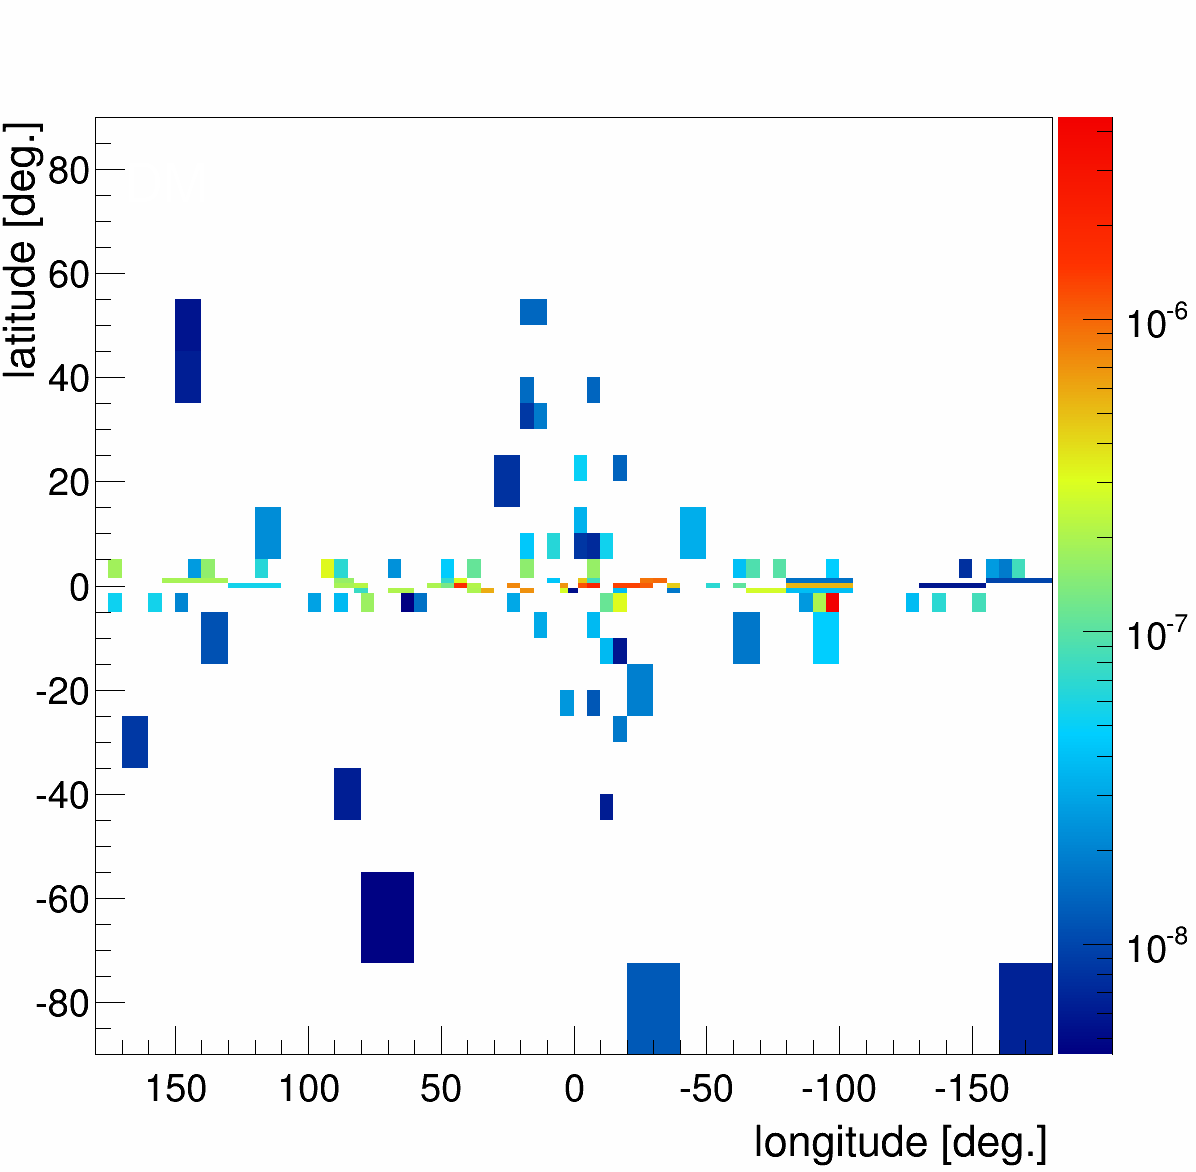
\includegraphics[width=.5\linewidth]{pic/discussion/DMlate_DM_distribution.png}
	\caption[DM distribution after fitting a MCR excess]{DM flux distribution when adding the DM component after fitting MCR. The initial MCR fit being already very good with a low $\chi^2$, DM cannot bring to much to the model. The adapted binning of 797 cones is used here because the statistics are too low in a one by one degree binning to show the DM contribution.}
	\label{fig:DMlate_distribution}
\end{figure}
%\newpage
%\section{How do these results fit in context}
%%How do they fit in context:
%%	-DM explanation
%%		-Best mass around 50 GeV
%%		-Increase goodness of fit
%%		-Not spherical at all
%%		-Follows CO map when there is no reason to do it
%%	-MSP explanation
%%		-Spectra too soft at low energies.
%%		-Same problem than with DM.
%%		
%%	-What's new?





